\documentclass[hyperref]{ctexart}
\usepackage[left=2.50cm, right=2.50cm, top=2.50cm, bottom=2.50cm]{geometry} %页边距
\usepackage{helvet}
\usepackage{amsmath, amsfonts, amssymb} % 数学公式、符号
\usepackage[english]{babel}
\usepackage{graphicx}   % 图片
\usepackage{url}        % 超链接
\usepackage{bm}         % 加粗方程字体
\usepackage{multirow}
\usepackage{booktabs}
\usepackage{algorithm}
\usepackage{algorithmic}
\usepackage{fancyhdr} %设置页眉、页脚
\pagestyle{fancy}
\lhead{}
\chead{}
\lfoot{}
\cfoot{}
\rfoot{}
\usepackage{hyperref} %bookmarks
\hypersetup{colorlinks, bookmarks, unicode} %unicode
\usepackage{multicol}
\title{\textbf{宇宙线$\mu$子平均寿命测量}}
\author{\sffamily 赵宇航}
\date{}
\begin{document}
\maketitle
\indent{\bf 摘要: }本实验测量了宇宙线$\mu$子的平均寿命,以及其随角度的变化关系。\\	
%\begin{multicols}{2}
\CTEXsetup[format={\Large\bfseries}]{section}
	\section{实验目的}
	1.加深宇宙线$\mu$子性质的认识;
	
	2.掌握宇宙线$\mu$子平均寿命的测量原理;

	\section{实验原理}
	宇宙线中的$\mu$子主要是由宇宙线中的$\pi$介子衰变($\pi^- \rightarrow \mu^- + \overline{\nu_{\mu}}$,$\pi^+\rightarrow \mu^+ + \nu_{\mu}$)产生的.大部分的 子产生在约 15 km 的高空,由于$\mu$子不参与强相互作用,因而具有较强的穿透力.海平面上$\mu$子的通量近似为$1 \sim 2 cm^{-2} min^{-1}$,平均能量约为4GeV 。$\mu$子带有 1 个单位的电荷,其质量$为105.658MeV /c^2 $,平均寿命约 2.197us 。

	宇宙线中的 $\mu$子通过塑料闪烁体时,主要的能量损失方式是电离能损,并伴随库仑散射.高能量 $\mu$子可直接从闪烁体中穿出,并在径迹周围产生电子及荧光光子等次级粒子;一些较低能量 $\mu$ 子在闪烁体中停止后,可以自由衰变,也可能与物质的原子核发生作用被俘获而消失.其发生衰变如下:
	\begin{equation}
	\mu^- \rightarrow e + \overline{V_e} + V_{\mu}
	\end{equation}

	衰变中产生的电子( e )继续与闪烁体发生作用损失能量,并使闪烁体分子激发,而电子反中微子$\overline{V_e} $和$\mu$子中微子$V_{\mu} $直接穿出.塑料闪烁体中受激发的分子在极短的时间内(约$10^{-10} s$ )退激发并发射荧光(荧光波长在$350 \sim 500nm $之间),荧光通过光电倍增管光电转换放大而输出电信号,这个信号将作为$\mu$ 子的“到达”信号.当停止在闪烁体内的 $\mu$ 子发生衰变,产生的电子被闪烁探测器探测,形成$\mu$子“衰变”的信号。“到达”探测器的信号与 $\mu$ 子“衰变”的信号的时间间隔, 即为 $\mu$ 子 1 次衰变的寿命.由于微观粒子的衰变具有一定的统计性,因此实验上是通过测量时间差的分布,进而计算得到 $\mu$子的平均寿命。

	宇宙线中$\mu$ 子的通量很低,每次击中探测器的事例可以看成单$\mu$子事例.设$\mu$子的平均寿命为$\tau$ ,第i 个$\mu$ 子的产生时间为$t_i$ ,则相对公共的时间零点, $\mu$子在时刻t 衰变概率为
	\begin{equation}
	D_i(t)=\frac{e^{-(t-t_i)/\tau}}{\tau}
	\end{equation}

	如果第i 个 $\mu$子到达闪烁探测器的时刻为$T_i$ ,那么时间间隔$\triangle T$内,这个 $\mu$子衰变的概率是:
	\begin{equation}
	P = \int_{T}^{T+\triangle T} D_i(t)dt = \int_{T}^{T+\triangle T} \frac{e^{-(t-t_i)/\tau}}{\tau}dt = K-Ke^{-\triangle T/ \tau}
	\end{equation}

	式中 $ K=e^{-(T-t_i)/\tau}$ 。如果实验共测量到M 个 $\mu$子衰变事例,则在时间差$\triangle T$以内, 衰变的总  $\mu$子数 N 为
	\begin{equation}
	N = \sum_{i=1}^{M} K_i(1- e^{-\triangle T/\tau})=K(1- e^{-\triangle T/\tau})
	\end{equation}

	式中$K=\sum_{i=1}^{M}$。

	可见在$\triangle T$ 时间内 $\mu$子衰变数随时间同样服从指数规律.实验上通过记录确定时间间隔内的$\mu$子衰变事例数,利用指数函数拟合方法,可以求得$\mu$子衰变的平均寿命$\tau$ 。

	\section{实验结果}
	根据实验所测的数据,知$\mu$子衰变的平均寿命为$2.2014 \pm 0.0191\mu s$。

	我们只需要研究一个分布规律,所以以单位时间通过粒子数代替单位时间通量,其随探测器角度改变分布如下表所示
	$$\begin{tabular}{|c|c|c|c|c|c|c|c|c|c|c|c|c|}
	\hline
	探测器角度 & 0 & 1 & 2 & 3 & 4 & 5 & 6 & 7 & 8 & 9  \\ \hline
	单位时间粒子数 & 2.910 & 0.089 & 0.196 & 0.335 & 0.431 & 0.475 & 0.497 & 0.712 & 0.848 & 0.781   \\ \hline
	探测器角度 & 10 & 20 & 25 & 30 & 35 & 40 & 45 & 50 & 55 & 60    \\ \hline
	单位时间粒子数 & 0.962 & 1.453 & 1.199 & 1.632 & 1.176 & 1.210 & 0.962 & 1.175 & 0.806 & 0.757  \\ \hline
	\end{tabular}$$

	\begin{figure}[H]
	\begin{minipage}{0.5\linewidth}
	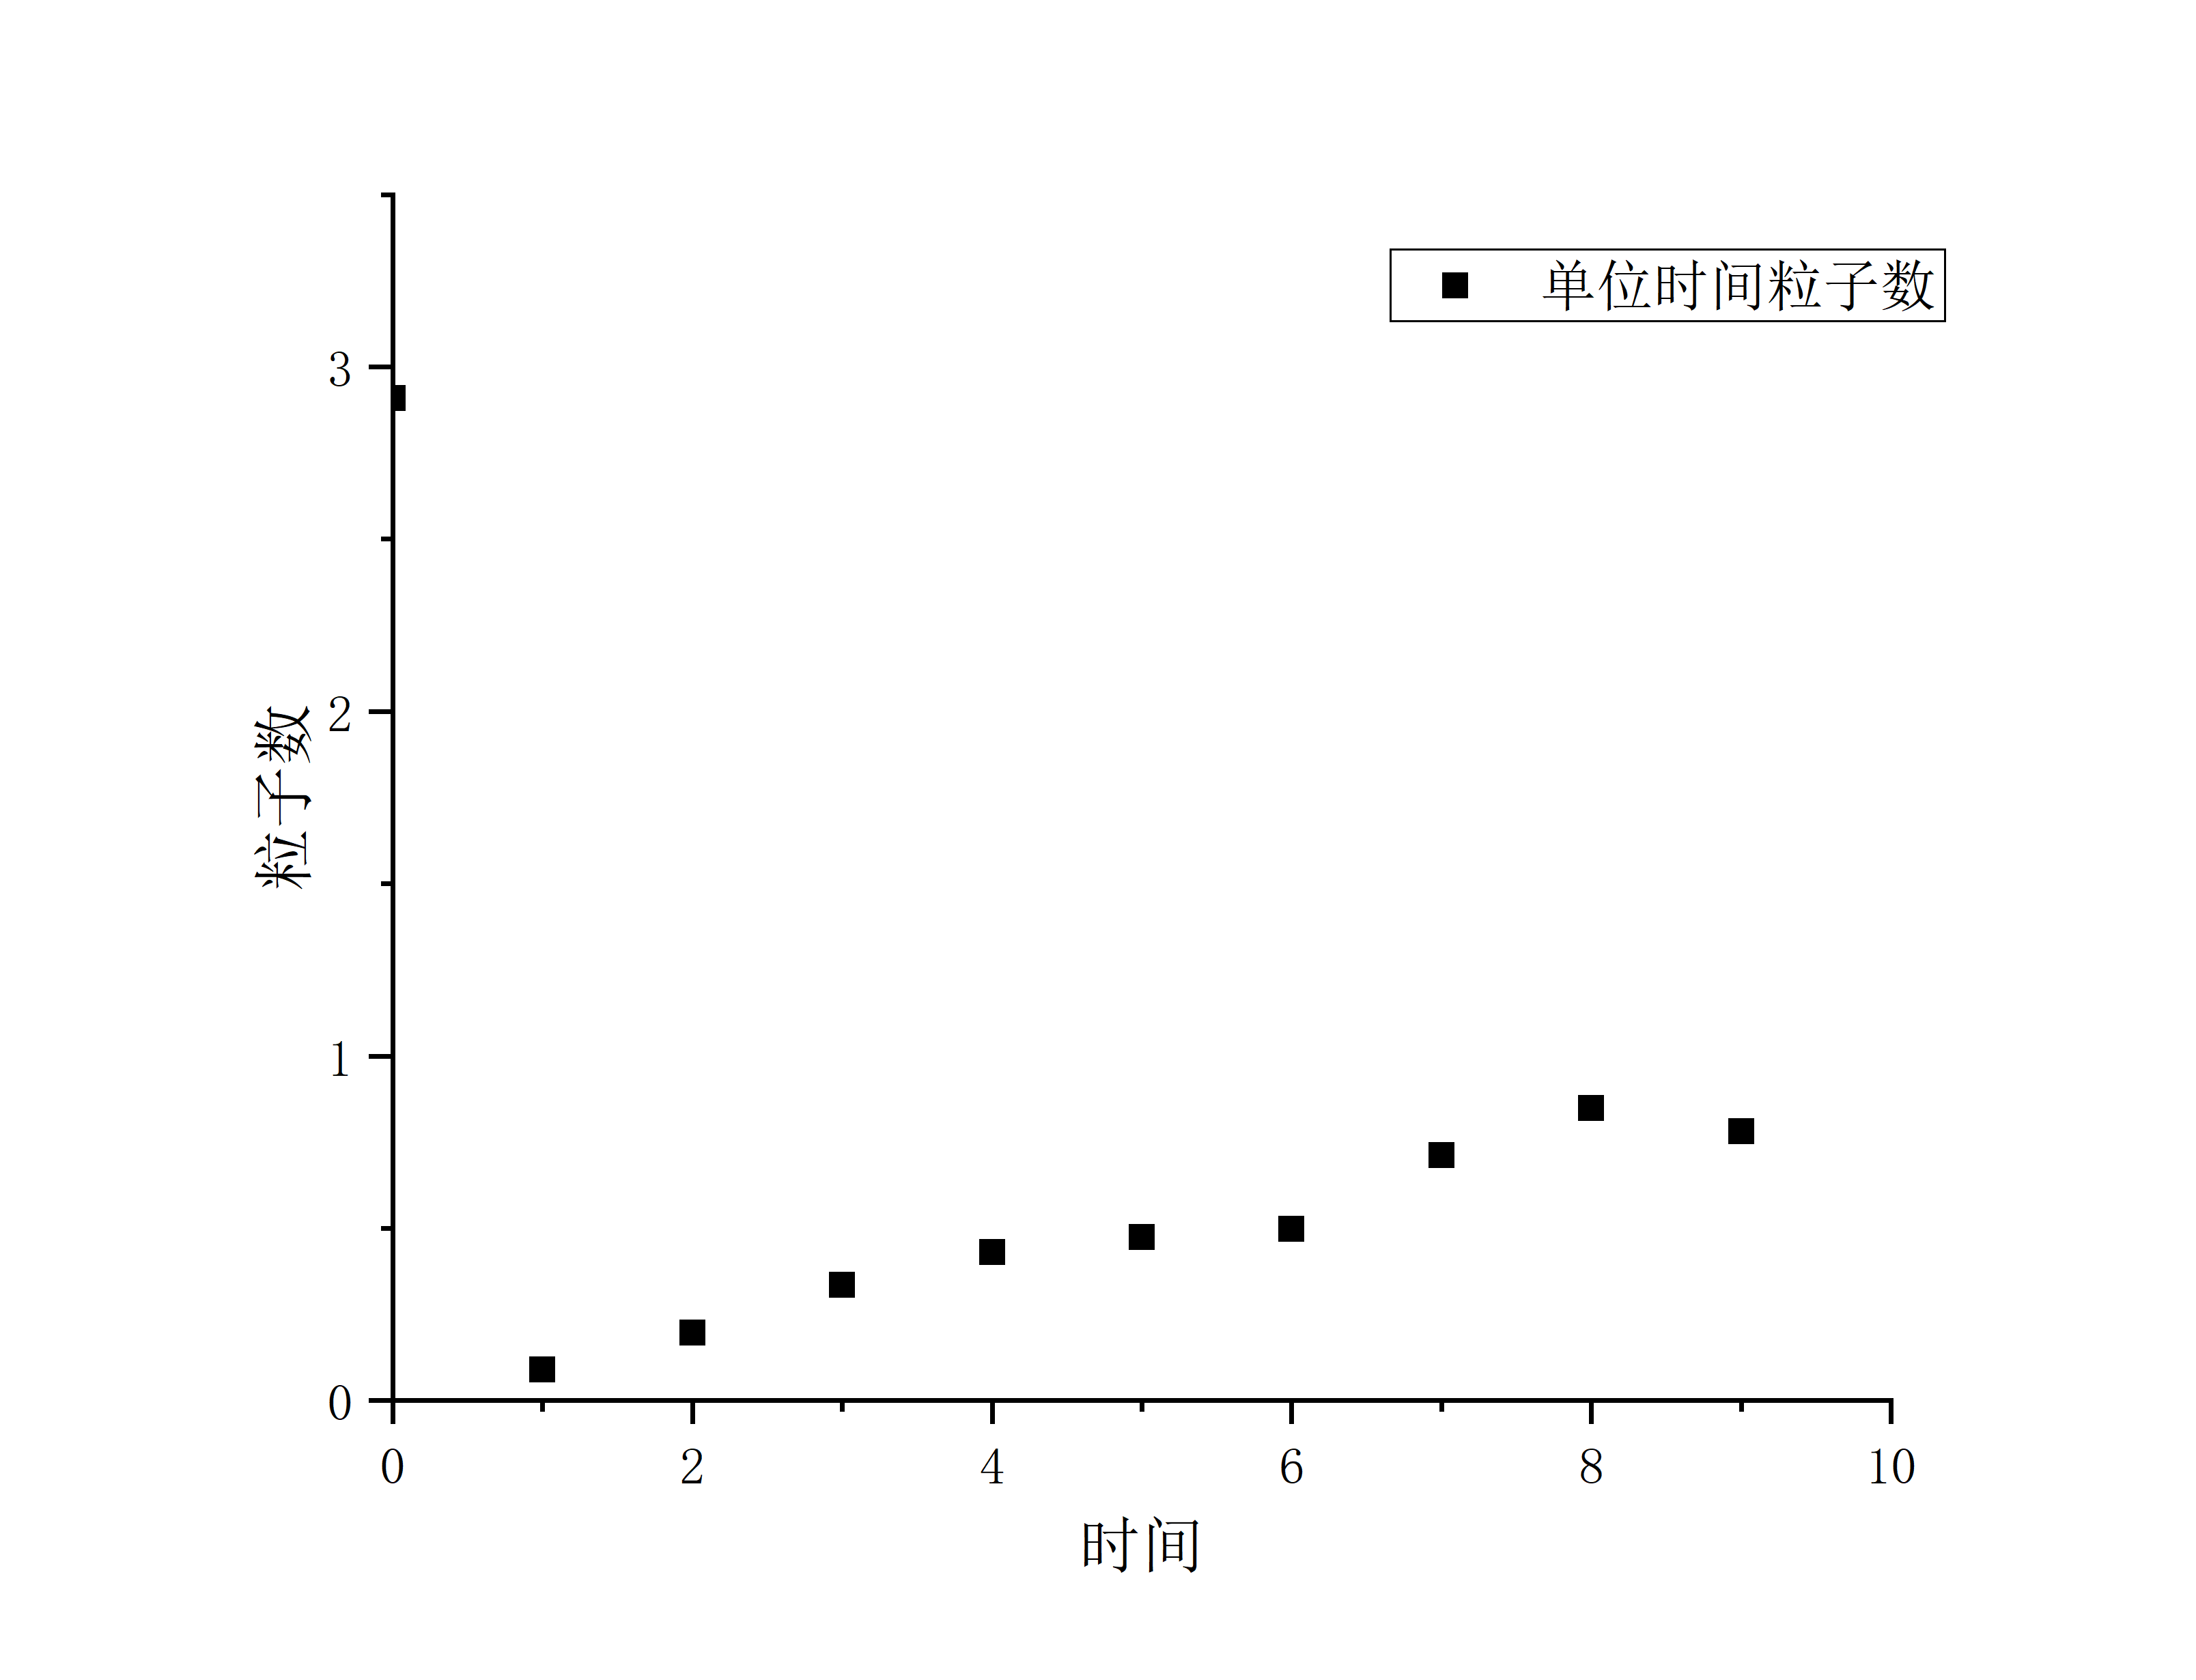
\includegraphics[scale=0.3]{t11}
	\end{minipage}
	\begin{minipage}{0.25\linewidth}
	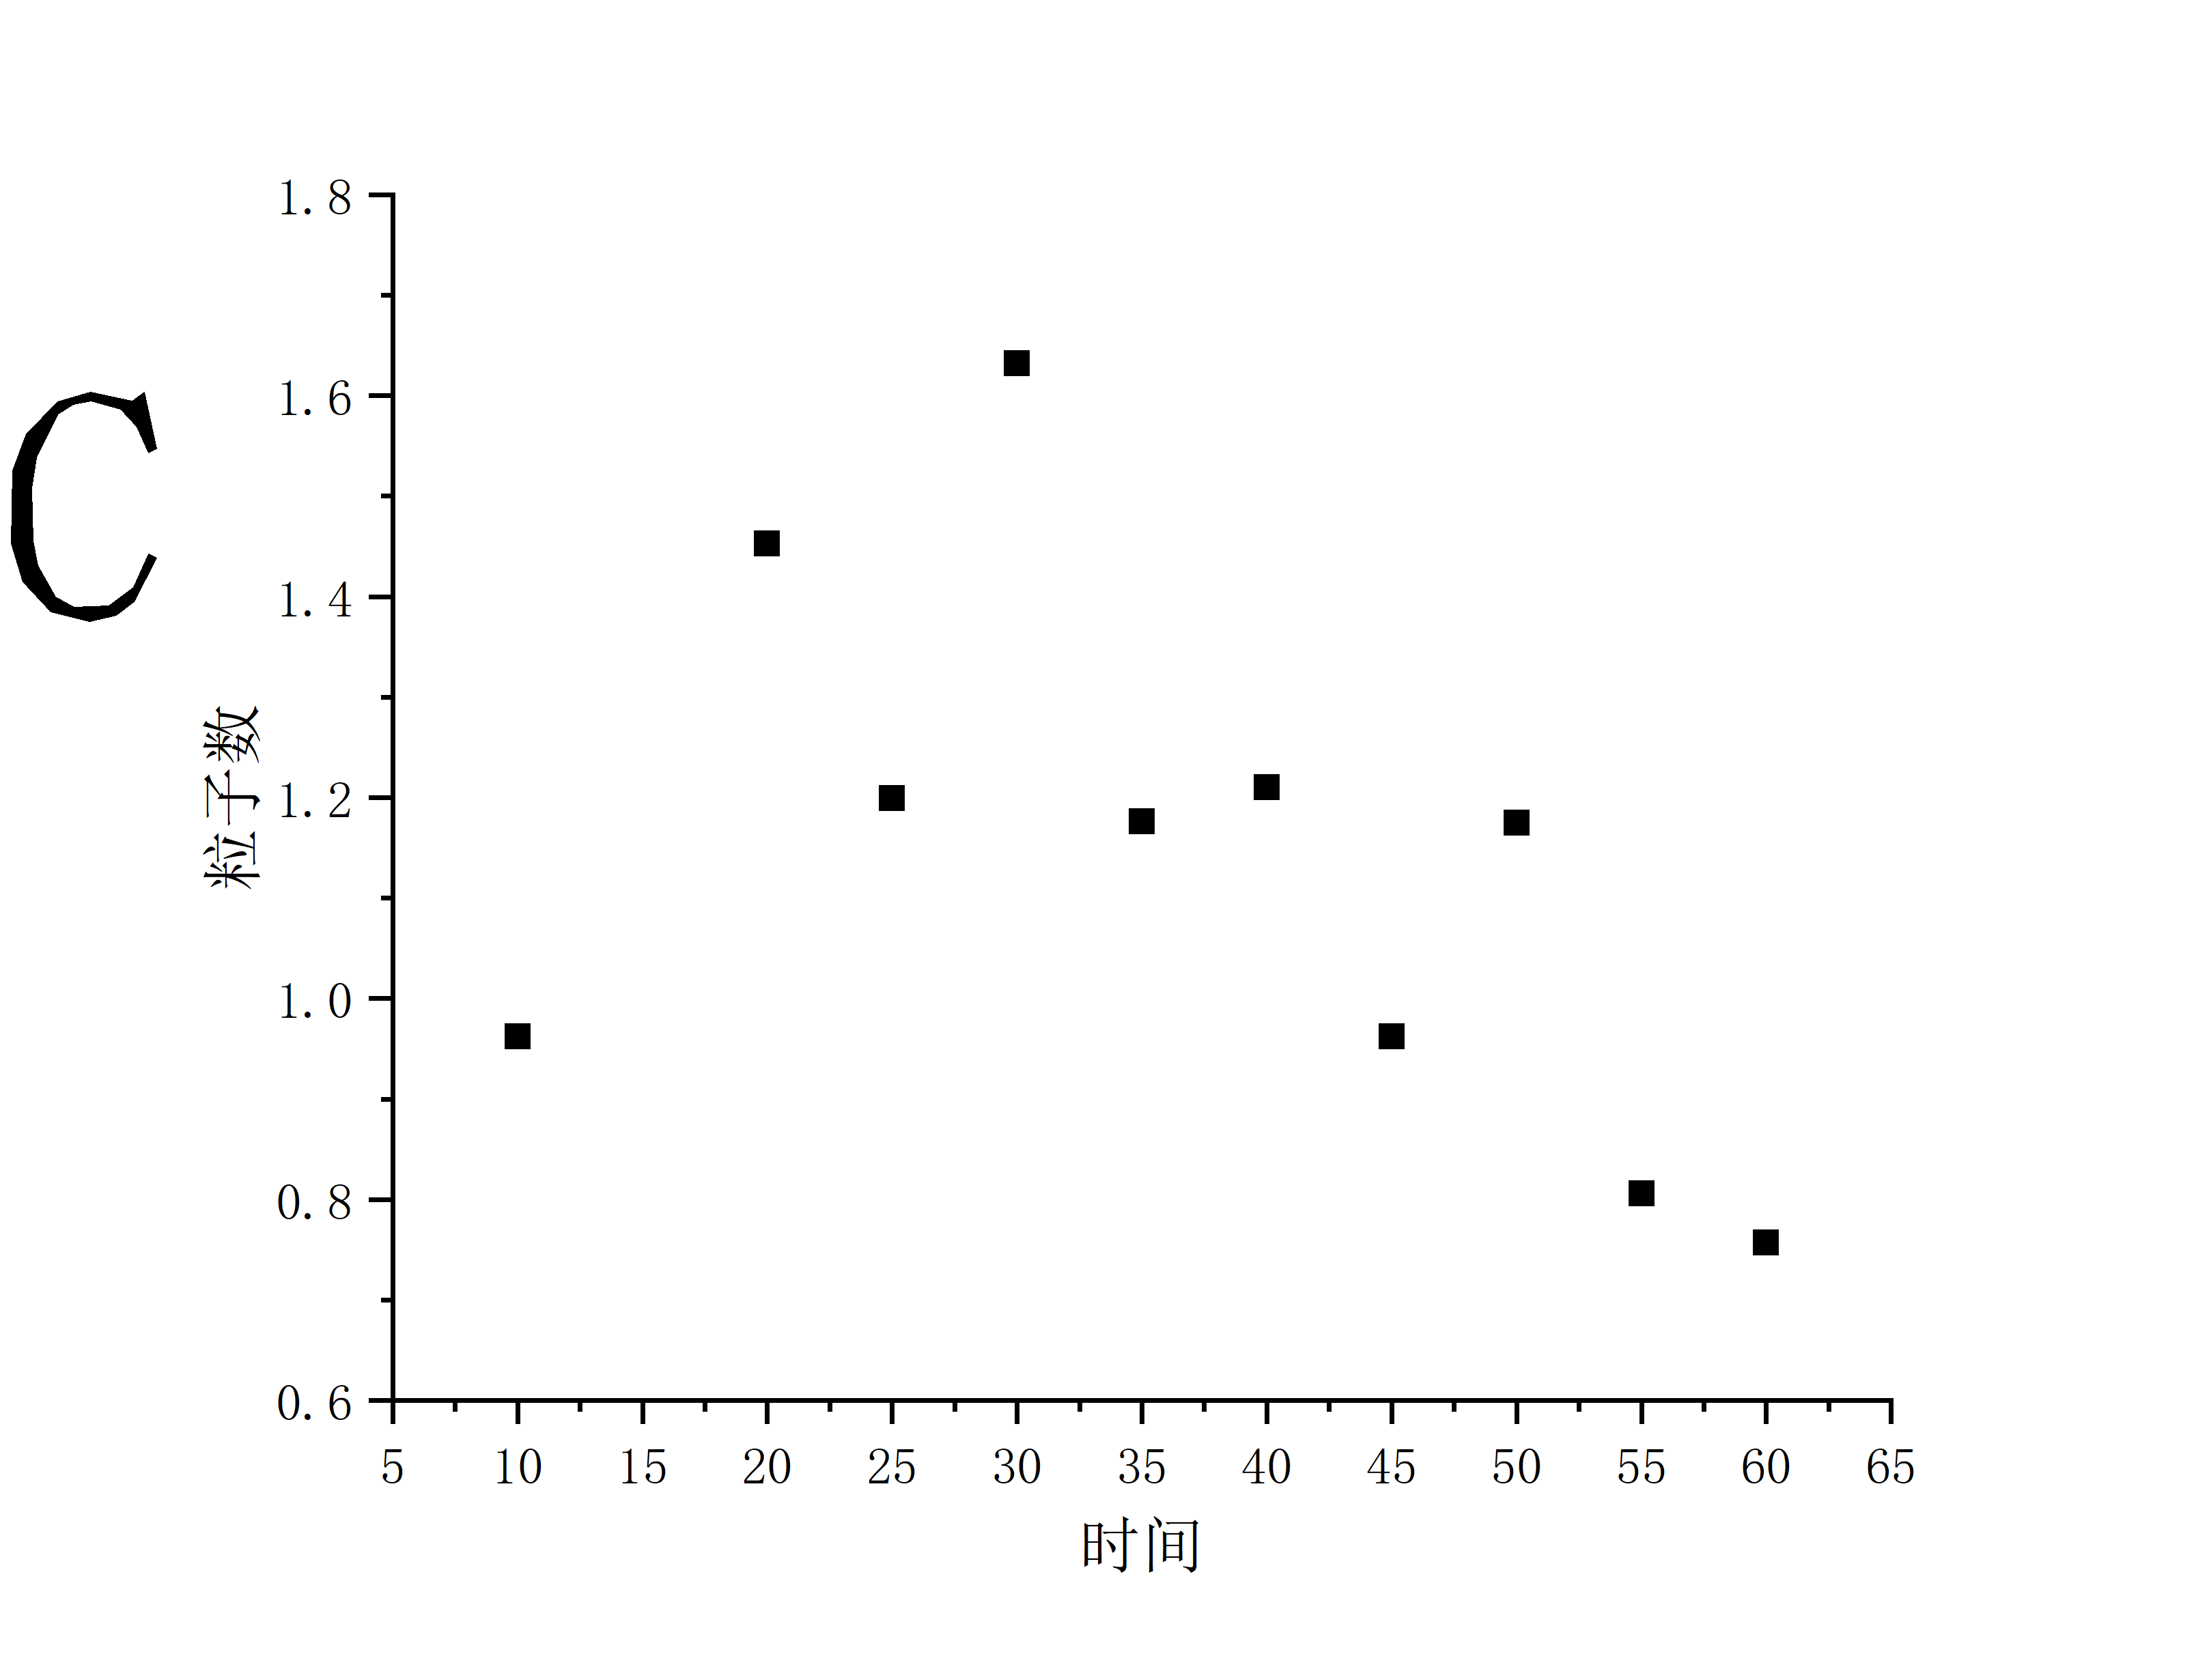
\includegraphics[scale=0.3]{t12}
	\end{minipage}
	\end{figure}

	在探测器角度比较小的时候,$\mu$子单位时间通量和探测器角度成正比;在探测器角度比较大的时候,$\mu$子单位时间通量大致先增加后减小,在$30^{\circ}$达到最大值。。






	\section{讨论}
	所有的$\mu$子全同,它们以同样地概率衰变,所以大量$\mu$子绘出的寿命曲线从统计上看就有确定的分布。
	
	实验中所取的单位时间内,只有不到2个粒子发生了衰变。可见,如果我们选取一定的时间间,只以到达信号与衰变信号小于这个间隔的取例,那么在间隔时间内连续两个粒子衰变的概率会达到二次小量(大约$10^{-4}$),可以忽略不计。






%\end{multicols}
\end{document}